% ============================================================
%  NEORV32 Accelerator for Cryptography
%  Ascon-AEAD128 Hardware Accelerator
%  Requirements & Design Document
%  Author: Mohammadi Masoudi Ramin
% ============================================================
\documentclass[11pt,a4paper]{article}

\usepackage[T1]{fontenc}
\usepackage[utf8]{inputenc}
\usepackage[margin=2.5cm]{geometry}
\usepackage{hyperref}
\usepackage{booktabs}
\usepackage{longtable}
\usepackage{array}
\usepackage{xcolor}
\usepackage{colortbl}
\usepackage{listings}
\usepackage{tikz}
\usetikzlibrary{arrows.meta,positioning,shapes.geometric,shapes.misc,calc,fit,automata}
\usepackage{amsmath}
\usepackage{amssymb}
\usepackage{graphicx}
\usepackage{fancyhdr}
\usepackage{titlesec}
\usepackage{enumitem}
\usepackage{float}
\usepackage{multirow}
\usepackage{tabularx}
\usepackage{tcolorbox}
\tcbuselibrary{skins,breakable}

% -- Colours ---------------------------------------------------
\definecolor{docblue}{RGB}{0,51,102}
\definecolor{doclblue}{RGB}{0,85,128}
\definecolor{reqbg}{RGB}{235,244,255}
\definecolor{reqframe}{RGB}{70,100,150}
\definecolor{nfrbg}{RGB}{240,255,240}
\definecolor{nfrframe}{RGB}{40,120,70}
\definecolor{codebg}{RGB}{247,247,247}
\definecolor{tabhead}{RGB}{0,51,102}
\definecolor{rowalt}{RGB}{243,247,255}
\definecolor{warnbg}{RGB}{255,251,230}
\definecolor{warnframe}{RGB}{170,120,0}
\definecolor{stateblue}{RGB}{0,70,140}
\definecolor{statefill}{RGB}{220,232,250}

\hypersetup{
  colorlinks=true, linkcolor=docblue, urlcolor=doclblue, citecolor=docblue,
  pdftitle={NEORV32 Ascon-AEAD128 Hardware Accelerator: Requirements and Design},
  pdfauthor={Mohammadi Masoudi Ramin}
}

\titleformat{\section}
  {\Large\bfseries\color{docblue}}{\thesection}{1em}{}
  [\color{docblue}\rule{\linewidth}{0.6pt}]
\titleformat{\subsection}
  {\large\bfseries\color{docblue}}{\thesubsection}{1em}{}
\titleformat{\subsubsection}
  {\normalsize\bfseries\color{doclblue}}{\thesubsubsection}{1em}{}

\pagestyle{fancy}\fancyhf{}
\fancyhead[L]{\small\color{docblue}\textbf{NEORV32 Ascon-AEAD128 Hardware Accelerator}}
\fancyhead[R]{\small\color{docblue}Requirements \& Design Document}
\fancyfoot[C]{\small\thepage}
\renewcommand{\headrulewidth}{0.4pt}

\lstdefinelanguage{myc}{
  morekeywords={int,uint8_t,uint32_t,void,const,return,if,while,static,inline},
  morecomment=[l]{//}, morecomment=[s]{/*}{*/},
  morestring=[b]"
}
\lstset{
  backgroundcolor=\color{codebg},
  basicstyle=\ttfamily\footnotesize,
  breaklines=true, frame=single, rulecolor=\color{gray!35},
  numbers=left, numberstyle=\tiny\color{gray!55},
  keywordstyle=\color{docblue}\bfseries,
  commentstyle=\color{gray!65}\itshape,
  stringstyle=\color{doclblue},
  xleftmargin=2em, framexleftmargin=2em,
  aboveskip=8pt, belowskip=6pt
}

\newcommand{\req}[3]{%
  \begin{tcolorbox}[
    enhanced, colback=reqbg, colframe=reqframe,
    arc=2pt, boxrule=0.5pt,
    left=6pt, right=6pt, top=3pt, bottom=3pt,
    attach boxed title to top left={yshift=-2mm, xshift=8pt},
    boxed title style={colback=reqframe, arc=2pt, boxrule=0pt,
                       left=4pt, right=4pt, top=2pt, bottom=2pt},
    title={\small\bfseries\color{white}#1\enspace\textbar\enspace\textit{#2}},
    before upper={\small}
  ]
  #3
  \end{tcolorbox}\vspace{3pt}}

\newcommand{\nfr}[3]{%
  \begin{tcolorbox}[
    enhanced, colback=nfrbg, colframe=nfrframe,
    arc=2pt, boxrule=0.5pt,
    left=6pt, right=6pt, top=3pt, bottom=3pt,
    attach boxed title to top left={yshift=-2mm, xshift=8pt},
    boxed title style={colback=nfrframe, arc=2pt, boxrule=0pt,
                       left=4pt, right=4pt, top=2pt, bottom=2pt},
    title={\small\bfseries\color{white}#1\enspace\textbar\enspace\textit{#2}},
    before upper={\small}
  ]
  #3
  \end{tcolorbox}\vspace{3pt}}

\newcommand{\warn}[1]{%
  \begin{tcolorbox}[
    enhanced, colback=warnbg, colframe=warnframe,
    arc=2pt, boxrule=0.5pt, left=6pt, right=6pt, top=3pt, bottom=3pt,
    before upper={\small}
  ]
  \textbf{\color{warnframe}Important:} #1
  \end{tcolorbox}\vspace{3pt}}

\newcolumntype{L}[1]{>{\raggedright\arraybackslash}p{#1}}
\newcolumntype{C}[1]{>{\centering\arraybackslash}p{#1}}
\newcommand{\thead}[1]{\cellcolor{tabhead}\color{white}\textbf{\small #1}}
\newcommand{\trow}{\rowcolor{rowalt}}

\setlength{\parskip}{5pt}
\setlength{\parindent}{0pt}
\setlist[itemize]{noitemsep, topsep=2pt}
\setlist[enumerate]{noitemsep, topsep=2pt}

% ============================================================
\begin{document}
% ============================================================

\begin{titlepage}
\centering
\vspace*{1.8cm}
{\color{docblue}\rule{\linewidth}{2pt}}\vspace{6pt}
{\color{docblue}\rule{\linewidth}{0.4pt}}
\vspace{1.5cm}

{\Huge\bfseries\color{docblue} NEORV32 Accelerator for Cryptography}\\[0.6em]
{\LARGE\bfseries\color{docblue} Ascon-AEAD128 Hardware Accelerator}\\[0.5em]
{\Large\color{doclblue} Requirements \& Design Document}

\vspace{1.5cm}
{\color{docblue}\rule{\linewidth}{0.4pt}}\vspace{6pt}
{\color{docblue}\rule{\linewidth}{2pt}}
\vspace{2cm}

\begin{tabular}{@{}ll@{}}
  \toprule
  \textbf{Author}          & Mohammadi Masoudi Ramin \\[2pt]
  \textbf{Project Title}   & NEORV32 Accelerator for Cryptography \\[2pt]
  \textbf{Target Platform} & NEORV32 RISC-V SoC on Sipeed Tang Nano~9K \\[2pt]
  \textbf{FPGA Device}     & Gowin GW1NR-9 ($\approx$8876 LUTs, 6480 FFs) \\[2pt]
  \textbf{Integration}     & Custom Functions Subsystem (CFS) \\[2pt]
  \textbf{Algorithm}       & Ascon-AEAD128 per NIST SP~800-232 final (August 2025) \\[2pt]
  \textbf{HDL}             & Verilog (MIT licence) \\[2pt]
  \textbf{Document Rev.}   & 0.5 \\[2pt]
  \textbf{Date}            & \today \\
  \bottomrule
\end{tabular}

\vspace{2cm}
\begin{tcolorbox}[colback=reqbg, colframe=docblue, arc=4pt, boxrule=0.8pt,
  left=12pt, right=12pt, top=8pt, bottom=8pt]
\small\centering
This document defines the functional and non-functional requirements, hardware
architecture, register map, firmware programming model, verification strategy,
and validation plan for a hardware accelerator implementing the NIST
Ascon-AEAD128 authenticated encryption algorithm, integrated into a NEORV32
RISC-V processor system via the Custom Functions Subsystem.
\end{tcolorbox}
\end{titlepage}

\tableofcontents
\newpage

% ============================================================
\section{Introduction}
\label{sec:intro}
% ============================================================

\subsection{Purpose}

This document specifies the requirements and design of a hardware accelerator
implementing the Ascon-AEAD128 lightweight authenticated encryption algorithm.
It is the technical reference for the project \textit{NEORV32 Accelerator for
Cryptography}, covering algorithm background, system requirements, hardware
architecture, register-level programming model, verification and validation
approach, design challenges, and directions for future work.

\subsection{Project Goals}

The project explores four complementary areas:

\begin{enumerate}
  \item \textbf{Efficient hardware implementation of cryptographic primitives:}
        design a synthesisable Verilog implementation of the full
        Ascon-AEAD128 algorithm, structured for readability and FPGA resource
        efficiency.
  \item \textbf{CPU-to-accelerator interface:}
        expose the accelerator to software through a memory-mapped register
        interface compatible with the NEORV32 Custom Functions Subsystem.
  \item \textbf{Correctness verification:}
        validate the RTL against a C golden model and a self-checking
        testbench suite covering primitives, AEAD core, and MMIO wrapper.
  \item \textbf{Performance benchmarking:}
        measure FPGA resource usage and compare hardware versus software
        throughput on the same processor.
\end{enumerate}

\subsection{Design Status}

This RASD describes the intended NEORV32 accelerator architecture and the
requirements that the implementation SHALL satisfy. The current development
flow uses a typed Python golden model, known-answer tests, generated Verilog
helpers, and Tang Nano~9K board bring-up infrastructure to reduce ambiguity
before final NEORV32 integration. Final synthesis, on-board validation, and
benchmark results will be reported in a separate development report.

\subsection{Scope}

The document covers the complete Ascon-AEAD128 accelerator:

\begin{itemize}
  \item The 320-bit Ascon permutation ($p[8]$ and $p[12]$).
  \item The AEAD128 mode: initialisation, associated-data absorption,
        plaintext/ciphertext streaming, finalisation, tag generation,
        and tag verification.
  \item The 32-bit MMIO register wrapper.
  \item The NEORV32 CFS VHDL integration wrapper.
  \item The C firmware driver.
\end{itemize}

\textbf{Out of scope:} ASIC physical implementation, ASIC synthesis, physical
layout, advanced side-channel countermeasures, DMA, multi-round-per-cycle
datapaths, and cryptographic certification. Architecture exploration beyond
the NEORV32 FPGA accelerator is documented separately in the development report.

\subsection{Assumptions and Constraints}

\begin{itemize}
  \item \textbf{Target board:} Sipeed Tang Nano~9K (Gowin GW1NR-9).
  \item \textbf{Integration point:} NEORV32 Custom Functions Subsystem.
  \item \textbf{HDL:} Verilog, synthesisable subset, no vendor primitives.
  \item \textbf{Development environment:} Nix flake providing Icarus Verilog,
        Yosys, GTKWave, GNU Make, Python~3.
  \item \textbf{Reference model:} the \texttt{ascon-c} C reference
        implementation is used as the golden model for vector generation
        and cross-validation. The Python scripts in \texttt{tools/} are
        supplementary utilities for bus-formatted vector printing.
  \item \textbf{Architecture:} iterative permutation, one round per clock
        cycle, prioritising area and design clarity over throughput.
\end{itemize}

\subsection{Normative Language}

The key words \textbf{SHALL}, \textbf{MUST}, \textbf{MUST NOT},
\textbf{SHOULD}, and \textbf{MAY} are interpreted as described in RFC~2119.

\subsection{References}

\begin{enumerate}
  \item NIST SP~800-232, \textit{Ascon-Based Lightweight Cryptography Standards for Constrained Devices}, final publication, August 2025.
  \item Dobraunig~et al., \textit{Ascon v1.2}, Journal of Cryptology, 2021.
  \item NEORV32 Processor Datasheet and User Guide, \url{https://stnolting.github.io/neorv32/}
  \item NEORV32 Custom Functions Subsystem documentation and CFS driver header.
  \item Sipeed Tang Nano~9K Schematic, Gowin GW1NR-9 Datasheet.
  \item Ascon-c reference implementation, \url{https://github.com/ascon/ascon-c}
\end{enumerate}


\subsection{Terminology}

\begin{tabular}{@{}lL{10cm}@{}}
  \toprule
  \textbf{Term} & \textbf{Definition} \\
  \midrule
  AEAD    & Authenticated Encryption with Associated Data \\
  CFS     & Custom Functions Subsystem --- NEORV32's memory-mapped accelerator interface \\
  IV      & Initialisation Vector --- 64-bit constant encoding Ascon-AEAD128 parameters \\
  KAT     & Known Answer Test \\
  LUT     & Look-Up Table, basic logic element of an FPGA \\
  FF      & Flip-Flop, single-bit synchronous storage element \\
  $p[n]$  & Ascon permutation applied for $n$ rounds \\
  Rate    & State bits absorbed or squeezed per block (128 bits = 16 bytes) \\
  Tag     & 128-bit authentication code appended to ciphertext \\
  RTL     & Register Transfer Level hardware description \\
  DUT     & Device Under Test \\
  \bottomrule
\end{tabular}

% ============================================================
\section{Background: Ascon-AEAD128}
\label{sec:background}
% ============================================================

\subsection{Why Ascon?}

Ascon is a family of lightweight cryptographic algorithms selected in 2023 as
NIST's primary standard for lightweight cryptography (SP~800-232). Its design
philosophy is simplicity: the 320-bit state fits in five 64-bit registers, and
the entire permutation is built from XOR, AND, NOT, and fixed rotations. This
makes it unusually compact in hardware while remaining secure at 128-bit
equivalent strength. Although the course assignment lists AES and SHA as
representative examples, Ascon-AEAD128 satisfies the same accelerator goal: it
is a standard cryptographic primitive implemented in hardware, exposed through
a CPU interface, verified against known-answer tests, and benchmarked against
software execution.

\subsection{State Representation}

The Ascon state is a vector of five 64-bit words:
\[
  S = (S_0 \;\|\; S_1 \;\|\; S_2 \;\|\; S_3 \;\|\; S_4)
\]

In the Verilog implementation this maps directly to a packed 320-bit bus:

\begin{center}
\begin{tabular}{@{}ll@{}}
  \toprule
  \textbf{State word} & \textbf{Bit slice} \\
  \midrule
  $S_0$ & \texttt{state[63:0]}     \\
  $S_1$ & \texttt{state[127:64]}   \\
  $S_2$ & \texttt{state[191:128]}  \\
  $S_3$ & \texttt{state[255:192]}  \\
  $S_4$ & \texttt{state[319:256]}  \\
  \bottomrule
\end{tabular}
\end{center}

Consequently, when a Verilog concatenation is used to build the packed bus,
the word order is reversed relative to the mathematical list:
\[
  \texttt{state} = \{S_4, S_3, S_2, S_1, S_0\}.
\]
External byte strings are interpreted little-endian within each 64-bit word:
byte~0 is the least-significant byte of $S_0$. For example, the byte sequence
\texttt{00 01 02 03 04 05 06 07} is represented as the integer word
\texttt{0x0706050403020100}. This distinction between byte-string display and
integer-word display is mandatory for all RTL, firmware, and test vectors.

\subsection{Permutation Structure}

Each round applies three sequential layers to the full 320-bit state:

\begin{enumerate}
  \item \textbf{Constant addition ($p_C$):} XOR an 8-bit round constant
        into the least-significant byte of $S_2$. The constant for round $i$
        of a $k$-round permutation is $c_i = \texttt{CONST}[16 - k + i]$,
        so $p[12]$ uses table indices 4--15 and $p[8]$ uses indices 8--15.
        The full table (index 0--15) is:
        \texttt{0x3c, 0x2d, 0x1e, 0x0f, 0xf0, 0xe1, 0xd2, 0xc3,
                0xb4, 0xa5, 0x96, 0x87, 0x78, 0x69, 0x5a, 0x4b}.

  \item \textbf{Substitution layer ($p_S$):} A non-linear 5-bit S-box is
        applied to all 64 vertical bit-slices of the state simultaneously,
        using the bit-sliced Boolean circuit given in Appendix~A of
        the NIST specification.

  \item \textbf{Linear diffusion layer ($p_L$):} Each word is updated
        by XOR-ing with two rotated copies of itself:
        \begin{align*}
          S_0 &\leftarrow S_0 \oplus \operatorname{rotR}(S_0,19) \oplus \operatorname{rotR}(S_0,28), \quad&
          S_1 &\leftarrow S_1 \oplus \operatorname{rotR}(S_1,61) \oplus \operatorname{rotR}(S_1,39), \\
          S_2 &\leftarrow S_2 \oplus \operatorname{rotR}(S_2, 1) \oplus \operatorname{rotR}(S_2, 6), \quad&
          S_3 &\leftarrow S_3 \oplus \operatorname{rotR}(S_3,10) \oplus \operatorname{rotR}(S_3,17), \\
          S_4 &\leftarrow S_4 \oplus \operatorname{rotR}(S_4, 7) \oplus \operatorname{rotR}(S_4,41).
        \end{align*}
\end{enumerate}

\subsection{AEAD128 Mode of Operation}

\subsubsection*{Phase~1 --- Initialisation}

\[
  S \;\leftarrow\; p^{12}\!\bigl(\,IV \;\|\; K \;\|\; N\,\bigr)
  \;\oplus\; \bigl(0^{192} \;\|\; K\bigr)
\]

The initialisation vector $IV = \texttt{0x00001000808c0001}$ encodes the
algorithm parameters ($k{=}128$, rate${=}128$, $a{=}12$, $b{=}8$).
After $p[12]$, the 128-bit key $K$ is XORed back into $S_3 \| S_4$. In the
RTL layout this corresponds to \texttt{state[319:192]}.

\subsubsection*{Phase~2 --- Associated Data}

Associated data $A$ is absorbed in 128-bit blocks:
for each block, XOR it into $(S_0 \| S_1)$, then apply $p[8]$.
The final partial block is padded by appending a 1-bit at the next bit position
followed by zeroes up to the rate boundary. After the last AD block, the
AEAD domain-separation bit is applied by toggling logical bit $S[319]$, which
corresponds to the most-significant bit of $S_4$ in the RTL vector.

\subsubsection*{Phase~3 --- Plaintext/Ciphertext}

For each 128-bit plaintext block $P_i$:
\[
  C_i = P_i \oplus (S_0 \| S_1),
  \qquad
  (S_0 \| S_1) \;\leftarrow\; C_i,
  \qquad\text{then apply }p[8].
\]

Decryption reverses the XOR to recover $P_i$ from $C_i$, while the state
absorbs $C_i$ identically to encryption. The final block uses the same
padding as AD.

\subsubsection*{Phase~4 --- Finalisation}

\[
  S \;\leftarrow\; p^{12}\!\bigl(S \;\oplus\; (0^{128} \;\|\; K \;\|\; 0^{64})\bigr),
  \qquad
  T \;=\; (S_3 \oplus K_0) \;\|\; (S_4 \oplus K_1)
\]

where $K_0 = K[63{:}0]$ and $K_1 = K[127{:}64]$. In the RTL state
layout this final key injection updates $S_2$ and $S_3$, and tag extraction
uses $S_3$ and $S_4$.

\subsection{Bus Byte Convention}

All 128-bit external buses use a \textbf{little-endian byte} layout:
\texttt{bus[7:0]}~=~byte~0. MMIO registers expose the low 32-bit word
first (\texttt{KEY0} holds key bytes 0--3). The C driver, testbenches,
and reference scripts all adhere to this convention; any deviation
produces incorrect ciphertext with no other diagnostic.

% ============================================================
\section{System Requirements}
\label{sec:requirements}
% ============================================================

\subsection{Functional Requirements}

\req{FR-001}{State representation}{%
  The design \textbf{SHALL} represent the Ascon state as five 64-bit words
  $S_0$--$S_4$ packed into a 320-bit vector using the NIST little-endian
  state convention: $S_0$ at bits \texttt{[63:0]}, $S_1$ at
  \texttt{[127:64]}, $S_2$ at \texttt{[191:128]}, $S_3$ at
  \texttt{[255:192]}, and $S_4$ at \texttt{[319:256]}.}

\req{FR-002}{Round constant addition}{%
  The design \textbf{SHALL} XOR the 8-bit round constant (selected by index
  $16 - \textit{rounds} + i$) into the least-significant byte of $S_2$.
  Constants \textbf{SHALL} match NIST SP~800-232, Table~5, exactly.}

\req{FR-003}{Substitution layer}{%
  The design \textbf{SHALL} implement the Ascon S-box as a bit-sliced Boolean
  circuit applied to all 64 vertical bit-slices of the state in parallel.
  The truth table \textbf{SHALL} agree with the reference specification for all 32
  possible inputs.}

\req{FR-004}{Linear diffusion layer}{%
  The design \textbf{SHALL} implement $p_L$ using the XOR-rotation amounts
  specified for each of the five 64-bit state words.}

\req{FR-005}{One combinational round}{%
  The design \textbf{SHALL} compose one complete round as
  $p_L(p_S(p_C(\text{state})))$ in a purely combinational block, with no
  internal state registers.}

\req{FR-006}{Iterative permutation engine}{%
  The design \textbf{SHALL} implement an iterative engine accepting a
  \texttt{rounds\_i} parameter in the range 1--16, advancing one round per
  clock cycle, and asserting \texttt{done\_o} for exactly one cycle on
  completion.}

\req{FR-007}{Permutation variants}{%
  Ascon-AEAD128 \textbf{SHALL} use $p[12]$ during initialisation and
  finalisation, and $p[8]$ during data absorption. The round-constant
  start index is computed as $16 - k$ for a $k$-round permutation.}

\req{FR-008}{Authenticated encryption}{%
  The design \textbf{SHALL} implement the Ascon-AEAD128 encryption mode
  per NIST SP~800-232: initialisation, AD absorption with padding and
  domain separation, plaintext absorption with ciphertext output, and
  finalisation with 128-bit tag generation.}

\req{FR-009}{Authenticated decryption}{%
  The design \textbf{SHALL} implement Ascon-AEAD128 decryption, recovering
  plaintext from ciphertext and performing a constant-time 128-bit tag
  comparison. The \texttt{tag\_ok\_o} output \textbf{SHALL} be high if and
  only if all 128 tag bits match.}

\req{FR-010}{Input length support}{%
  The design \textbf{SHALL} correctly handle: zero-length AD, zero-length
  message, inputs that are exact multiples of 16 bytes, and partial final
  blocks of 1--15 bytes for both AD and message.}

\req{FR-011}{Padding and domain separation}{%
  Padding (1-bit append at the rate boundary) and AD/message domain
  separation \textbf{SHALL} be applied by the hardware internally, without
  any software pre-processing.}

\req{FR-012}{Tag verification}{%
  The tag comparison in decryption \textbf{SHALL} be implemented as a
  constant-time bitwise AND-reduction over all 128 bits. It \textbf{MUST NOT}
  short-circuit on any earlier bit match or mismatch.}

\req{FR-013}{CPU register interface}{%
  The design \textbf{SHALL} expose a 32-bit memory-mapped interface compatible
  with the NEORV32 CFS bus: one-cycle pipelined acknowledge, full-word-only
  writes enforced at the hardware level, and 8-bit address decoding within the
  256-byte CFS window.}

\req{FR-014}{NEORV32 CFS integration}{%
  The design \textbf{SHALL} include a VHDL wrapper (\texttt{neorv32\_cfs.vhd})
  presenting the standard NEORV32 CFS entity ports (\texttt{bus\_req\_i},
  \texttt{bus\_rsp\_o}, \texttt{irq\_o}) and instantiating the Verilog MMIO
  core as a component.}

\req{FR-015}{Authenticated plaintext release}{%
  During decryption, plaintext blocks \textbf{SHALL NOT} be released outside
  the accelerator until the final authentication tag comparison succeeds.
  The design \textbf{SHALL} buffer recovered plaintext internally during
  decryption. If tag verification fails, the buffered plaintext \textbf{SHALL}
  be cleared or invalidated and \texttt{STATUS.TAG\_OK} \textbf{SHALL} remain
  de-asserted.}

\subsection{Non-Functional Requirements}

\nfr{NFR-001}{Synthesisability}{%
  The RTL \textbf{SHALL} elaborate under Yosys without errors, produce a
  valid JSON netlist, and contain no combinational loops and no
  vendor-specific primitives.}

\nfr{NFR-002}{Iterative architecture}{%
  The initial implementation \textbf{SHALL} apply one round per clock cycle.
  This choice favours area and design transparency; higher-performance
  variants are deferred to future work.}

\nfr{NFR-003}{Reproducible toolchain}{%
  The repository \textbf{SHALL} provide a \texttt{flake.nix} and
  \texttt{shell.nix} that supply a fully reproducible environment:
  Icarus~Verilog, Yosys, Graphviz, GTKWave, Python~3, and GNU~Make.}

\nfr{NFR-004}{Testbench suite}{%
  Self-checking testbenches \textbf{SHALL} be provided at the primitive,
  AEAD core, and MMIO wrapper levels. Each \textbf{SHALL} exit with a
  non-zero status code on failure and print an unambiguous \texttt{PASS}
  or \texttt{FAIL} line.}

\nfr{NFR-005}{Firmware driver correctness}{%
  The C driver \textbf{SHALL} implement a polling-based communication loop
  covering both encryption and decryption through a shared internal function.
  Interrupt-driven operation is optional.}

\nfr{NFR-006}{Core decoupling}{%
  \texttt{ascon\_aead128\_core} \textbf{SHALL} contain no NEORV32-specific
  signals. All processor-side integration \textbf{SHALL} be confined to
  \texttt{ascon\_aead128\_mmio} and the VHDL wrapper, so the core can be
  reused with any 128-bit streaming interface.}

\nfr{NFR-007}{Timing determinism}{%
  Execution latency for a fixed input length \textbf{SHALL NOT} depend on
  the secret key value, plaintext, ciphertext, or tag content. The
  control path \textbf{SHALL} be identical for all data patterns.}

% ============================================================
\section{Hardware Architecture}
\label{sec:architecture}
% ============================================================

\subsection{Layered Design}

The design separates concerns into four layers:

\begin{enumerate}
  \item \textbf{Permutation primitive layer:}
        round constants, substitution, diffusion, a single combinational round,
        and the iterative permutation engine.
  \item \textbf{AEAD mode layer:}
        the streaming controller implementing all four algorithm phases.
  \item \textbf{MMIO layer:}
        the 32-bit register file and CFS bus interface.
  \item \textbf{Integration layer:}
        the VHDL CFS wrapper and C firmware driver.
\end{enumerate}

The call chain from firmware down to the permutation primitive is:

\begin{center}
\ttfamily\small
\begin{tabular}{@{}l@{}}
  NEORV32 C firmware \\
  \quad $\rightarrow$ CFS address space (NEORV32 bus) \\
  \quad\quad $\rightarrow$ neorv32\_cfs.vhd \\
  \quad\quad\quad $\rightarrow$ ascon\_aead128\_mmio.v \\
  \quad\quad\quad\quad $\rightarrow$ ascon\_aead128\_core.v \\
  \quad\quad\quad\quad\quad $\rightarrow$ ascon\_permutation\_iter.v \\
  \quad\quad\quad\quad\quad\quad $\rightarrow$ ascon\_round.v \\
\end{tabular}
\end{center}

\subsection{Top-Level Block Diagram}


\begin{figure}[H]
\centering
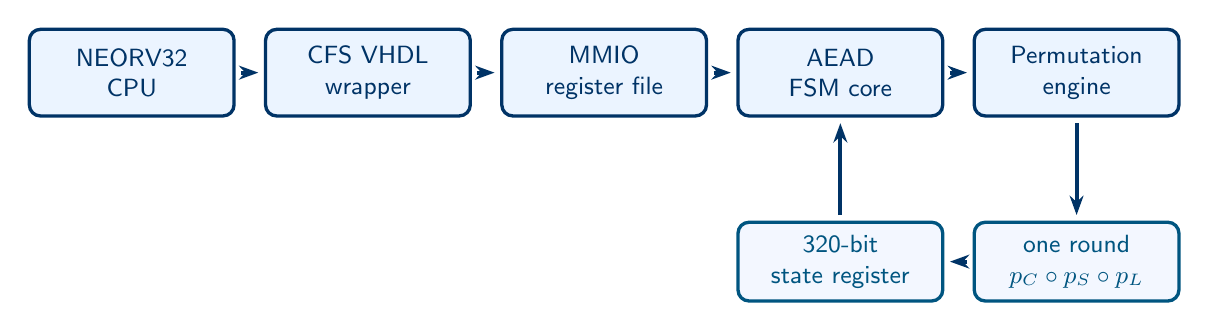
\begin{tikzpicture}[
  >=Stealth,
  B/.style = {draw=docblue, fill=reqbg, very thick, rounded corners=4pt,
              minimum width=2.6cm, minimum height=1.1cm,
              align=center, font=\small\sffamily, text=docblue},
  S/.style = {draw=doclblue, fill=rowalt, very thick, rounded corners=4pt,
              minimum width=2.6cm, minimum height=1.0cm,
              align=center, font=\small\sffamily, text=doclblue},
  arr/.style = {-{Stealth[length=7pt,width=5pt]},
                line width=1.4pt, color=docblue,
                shorten >=2pt, shorten <=2pt}
]

% Row A: five blocks, 3 cm pitch
\node[B] (CPU)  at ( 0,   0) {NEORV32\\CPU};
\node[B] (CFS)  at ( 3,   0) {CFS VHDL\\wrapper};
\node[B] (MMIO) at ( 6,   0) {MMIO\\register file};
\node[B] (CORE) at ( 9,   0) {AEAD\\FSM core};
\node[B] (PERM) at (12,   0) {Permutation\\engine};

% Row B: two sub-blocks under right pair
\node[S] (SREG) at ( 9,  -2.4) {320-bit\\state register};
\node[S] (RND)  at (12,  -2.4) {one round\\$p_C \circ p_S \circ p_L$};

% Call-chain (left to right)
\draw[arr] (CPU.east)  -- (CFS.west);
\draw[arr] (CFS.east)  -- (MMIO.west);
\draw[arr] (MMIO.east) -- (CORE.west);
\draw[arr] (CORE.east) -- (PERM.west);

% Permutation feedback loop (solid rectangle, no crossings)
\draw[arr] (PERM.south) -- (RND.north);
\draw[arr] (RND.west)   -- (SREG.east);
\draw[arr] (SREG.north) -- (CORE.south);

\end{tikzpicture}
\caption{System architecture.
The five design layers appear left to right: CPU, CFS VHDL wrapper,
MMIO register file, AEAD FSM core, and permutation engine.
Below, the 320-bit state register and combinational round function
form the per-cycle permutation feedback loop.
On completion, the AEAD core asserts an interrupt back to the CPU via \texttt{irq\_o}.}
\end{figure}


\subsection{Module Hierarchy}

\rowcolors{2}{rowalt}{white}
\begin{tabular}{@{}lL{4.5cm}L{7.5cm}@{}}
  \toprule
  \thead{Module} & \thead{File} & \thead{Responsibility} \\
  \midrule
  \texttt{ascon\_round\_constant}   & \texttt{ascon\_round\_constant.v}   &
    4-bit index to 8-bit constant ROM (16 entries per NIST SP~800-232 Table~5). \\
  \texttt{ascon\_constant\_add}     & \texttt{ascon\_constant\_add.v}     &
    XOR constant into LSB of $S_2$ ($p_C$ layer). \\
  \texttt{ascon\_sbox5}             & \texttt{ascon\_sbox5.v}             &
    Standalone 5-bit S-box truth-table LUT for formal equivalence checking. \\
  \texttt{ascon\_substitution}      & \texttt{ascon\_substitution.v}      &
    Bit-sliced Boolean $p_S$ applied to all 64 slices in parallel. \\
  \texttt{ascon\_diffusion}         & \texttt{ascon\_diffusion.v}         &
    XOR-rotation diffusion layer $p_L$ for $S_0$--$S_4$. \\
  \texttt{ascon\_round}             & \texttt{ascon\_round.v}             &
    One purely combinational round: $p_L(p_S(p_C(\cdot)))$. \\
  \texttt{ascon\_state\_reg}        & \texttt{ascon\_state\_reg.v}        &
    320-bit register with explicit load/update control and word outputs. \\
  \texttt{ascon\_permutation\_iter} & \texttt{ascon\_permutation\_iter.v} &
    Iterative engine: one round per clock, round counter, done signal. \\
  \texttt{ascon\_aead128\_core}     & \texttt{ascon\_aead128\_core.v}     &
    AEAD streaming FSM: all four algorithm phases, padding, tag comparison. \\
  \texttt{ascon\_aead128\_mmio}     & \texttt{ascon\_aead128\_mmio.v}     &
    32-bit register wrapper, bus decode, IRQ, CFS protocol. \\
  \texttt{neorv32\_cfs}             & \texttt{neorv32\_cfs.vhd}           &
    VHDL drop-in replacement for the NEORV32 CFS template. \\
  \bottomrule
\end{tabular}

\subsection{Permutation Engine}

The iterative engine (\texttt{ascon\_permutation\_iter}) processes one
combinational round per clock cycle:

\begin{itemize}
  \item On \texttt{start\_i}: latch \texttt{state\_i} and \texttt{rounds\_i};
        assert \texttt{busy\_o}; reset the round counter to zero.
  \item Each cycle: pass \texttt{state\_o} through one \texttt{ascon\_round}
        instance and write the result back into \texttt{state\_o};
        increment the round counter.
  \item When the counter reaches the target: de-assert \texttt{busy\_o},
        pulse \texttt{done\_o} for one cycle.
\end{itemize}

The first constant index is $16 - \texttt{rounds\_i}$, ensuring $p[12]$
selects table entries 4--15 and $p[8]$ selects entries 8--15, exactly as
the specification requires.

\textbf{Latency:} 12~cycles for $p[12]$; 8~cycles for $p[8]$.

\subsection{AEAD Core FSM}
\label{sec:fsm}

The AEAD controller (\texttt{ascon\_aead128\_core}) sequences through 16
states arranged in four algorithmic phases, each corresponding to a column
in Figure~\ref{fig:fsm}.


\begin{figure}[H]
\centering
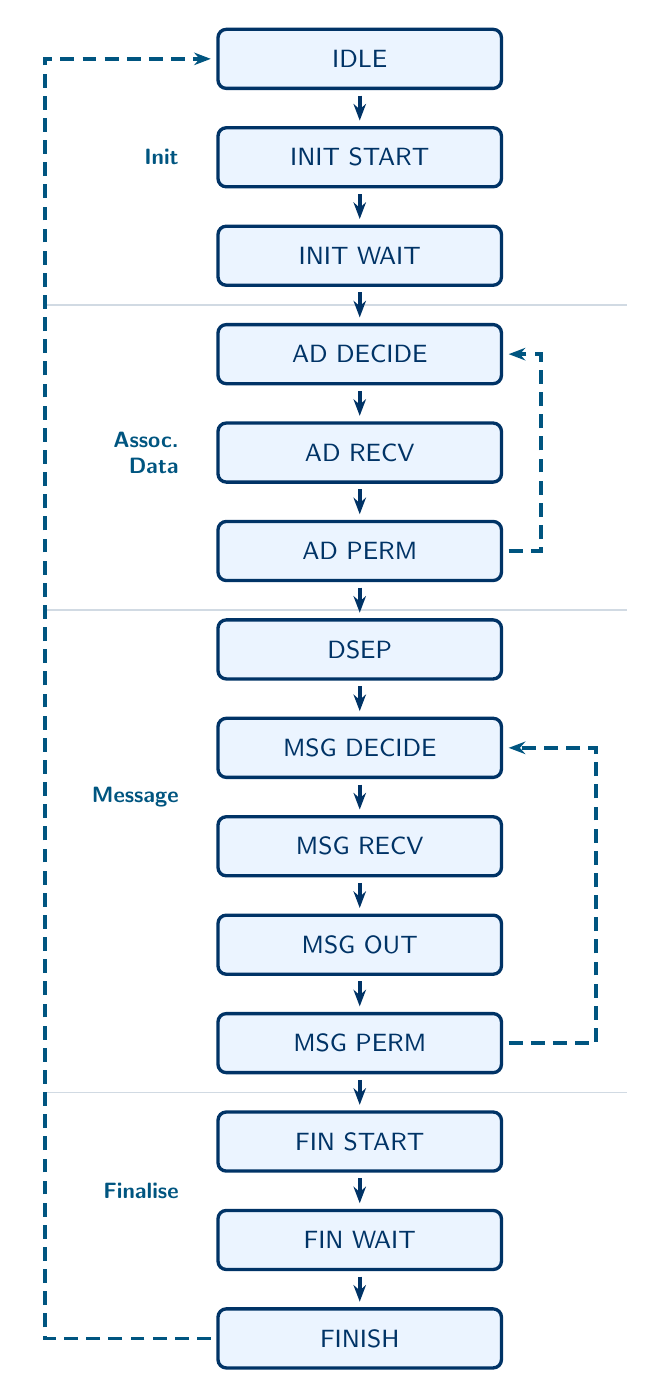
\begin{tikzpicture}[
  >=Stealth,
  % State box — slightly wider, compact height
  st/.style  = {draw=docblue, fill=reqbg, very thick, rounded corners=3pt,
                minimum width=3.6cm, minimum height=0.75cm,
                align=center, font=\small\sffamily, text=docblue},
  % Phase label
  ph/.style  = {font=\footnotesize\bfseries\sffamily, color=doclblue,
                align=right, text width=1.8cm},
  % Divider line
  div/.style = {color=docblue!18, line width=0.5pt},
  arr/.style = {-{Stealth[length=6pt,width=4.5pt]},
                line width=1.3pt, color=docblue,
                shorten >=2pt, shorten <=2pt},
  xarr/.style= {-{Stealth[length=6pt,width=4.5pt]},
                line width=1.3pt, color=doclblue, dashed,
                dash pattern=on 5pt off 3pt,
                shorten >=2pt, shorten <=2pt}
]

% States: single column at x=0, pitch = -1.25 cm
\node[st](IDL) at (0,  0.00){IDLE};
\node[st](IS)  at (0, -1.25){INIT START};
\node[st](IW)  at (0, -2.50){INIT WAIT};
\node[st](ADD) at (0, -3.75){AD DECIDE};
\node[st](AR)  at (0, -5.00){AD RECV};
\node[st](APS) at (0, -6.25){AD PERM};
\node[st](DS)  at (0, -7.50){DSEP};
\node[st](MDD) at (0, -8.75){MSG DECIDE};
\node[st](MR)  at (0,-10.00){MSG RECV};
\node[st](MO)  at (0,-11.25){MSG OUT};
\node[st](MP)  at (0,-12.50){MSG PERM};
\node[st](FPS) at (0,-13.75){FIN START};
\node[st](FPW) at (0,-15.00){FIN WAIT};
\node[st](FIN) at (0,-16.25){FINISH};

% Phase dividers (y midpoints between last/first state of adjacent phases)
\draw[div] (-4.0, -3.125) -- (3.4, -3.125); % Init | AD
\draw[div] (-4.0, -7.000) -- (3.4, -7.000); % AD   | MSG (incl DSEP)
\draw[div] (-4.0,-13.125) -- (3.4,-13.125); % MSG  | Fin

% Phase labels (left margin, at vertical centre of each band)
\node[ph] at (-3.2, -1.25) {Init};
\node[ph] at (-3.2, -5.00) {Assoc.\\Data};
\node[ph] at (-3.2, -9.38) {Message};
\node[ph] at (-3.2,-14.38) {Finalise};

% Sequential downward transitions
\draw[arr](IDL.south)--(IS.north);
\draw[arr](IS.south) --(IW.north);
\draw[arr](IW.south) --(ADD.north);
\draw[arr](ADD.south)--(AR.north);
\draw[arr](AR.south) --(APS.north);
\draw[arr](APS.south)--(DS.north);
\draw[arr](DS.south) --(MDD.north);
\draw[arr](MDD.south)--(MR.north);
\draw[arr](MR.south) --(MO.north);
\draw[arr](MO.south) --(MP.north);
\draw[arr](MP.south) --(FPS.north);
\draw[arr](FPS.south)--(FPW.north);
\draw[arr](FPW.south)--(FIN.north);

% Loop-back: AD PERM -> AD DECIDE (right hook, x = 2.3)
\coordinate(AL1) at (2.3, -6.25);
\coordinate(AL2) at (2.3, -3.75);
\draw[xarr](APS.east)--(AL1)--(AL2)--(ADD.east);

% Loop-back: MSG PERM -> MSG DECIDE (right hook, x = 3.0, outside AD hook)
\coordinate(ML1) at (3.0,-12.50);
\coordinate(ML2) at (3.0, -8.75);
\draw[xarr](MP.east)--(ML1)--(ML2)--(MDD.east);

% Return to IDLE (left side, x = -4.0)
\coordinate(RL1) at (-4.0,-16.25);
\coordinate(RL2) at (-4.0,  0.00);
\draw[xarr](FIN.west)--(RL1)--(RL2)--(IDL.west);

\end{tikzpicture}
\caption{AEAD core FSM. States appear top to bottom in execution order.
Phase boundaries are marked by light horizontal rules.
Dashed arcs on the right: per-block iteration loops back to
\texttt{AD~DECIDE} and \texttt{MSG~DECIDE}.
Dashed arc on the left: return to \texttt{IDLE} on completion.
Every state is described in full in the table below.}
\label{fig:fsm}
\end{figure}


\rowcolors{2}{rowalt}{white}
\begin{tabular}{@{}L{3.8cm}L{2cm}L{7.5cm}@{}}
  \toprule
  \thead{State} & \thead{Duration} & \thead{Action} \\
  \midrule
  \texttt{ST\_IDLE}             & ---      & Wait for \texttt{start\_i}. Latch key, nonce, mode, lengths, and expected tag. \\
  \texttt{ST\_INIT\_START}      & 1 cycle  & Load state $= (IV \| K \| N)$; pulse permutation with rounds~$= 12$. \\
  \texttt{ST\_INIT\_WAIT}       & 12 cycles & Wait for $p[12]$ done; XOR key into $S_3, S_4$. \\
  \texttt{ST\_AD\_DECIDE}       & 1 cycle  & Determine whether an AD block is pending or AD processing is complete. \\
  \texttt{ST\_AD\_RECV}         & varies   & Wait for a valid AD block; XOR into $(S_0 \| S_1)$ with padding logic. \\
  \texttt{ST\_AD\_PERM\_START}  & 1 cycle  & Pulse permutation with rounds~$= 8$. \\
  \texttt{ST\_AD\_PERM\_WAIT}   & 8 cycles & Wait for $p[8]$ done; update state register. \\
  \texttt{ST\_DSEP}             & 1 cycle  & XOR domain-separation word into $S_4$. \\
  \texttt{ST\_MSG\_DECIDE}      & 1 cycle  & Determine whether a message block or padding-only step is next. \\
  \texttt{ST\_MSG\_RECV}        & varies   & Accept PT/CT block; compute CT/PT output; update state with padding logic. \\
  \texttt{ST\_MSG\_OUT}         & 1+ cycles & Encryption: hold \texttt{data\_valid\_o} until the consumer acknowledges. Decryption: write recovered plaintext into the internal release buffer. \\
  \texttt{ST\_MSG\_PERM\_START} & 1 cycle  & Pulse $p[8]$ for a non-final message block. \\
  \texttt{ST\_MSG\_PERM\_WAIT}  & 8 cycles & Wait for $p[8]$ done. \\
  \texttt{ST\_FINAL\_PERM\_START} & 1 cycle & XOR key into state; pulse $p[12]$. \\
  \texttt{ST\_FINAL\_PERM\_WAIT}  & 12 cycles & Wait for $p[12]$ done; extract tag; compare tag. \\
  \texttt{ST\_FINISH}           & 1 cycle  & Assert \texttt{done\_o}; return to \texttt{ST\_IDLE}. \\
  \bottomrule
\end{tabular}

\subsection{Encryption vs.\ Decryption Data Flow}

\begin{center}
\rowcolors{2}{rowalt}{white}
\begin{tabular}{@{}lL{5.5cm}L{5.5cm}@{}}
  \toprule
  \thead{Step} & \thead{Encryption} & \thead{Decryption} \\
  \midrule
  Input (MSG phase)   & Plaintext $P$ from CPU & Ciphertext $C$ from CPU \\
  Output (MSG phase)  & $C_i = P_i \oplus (S_0 \| S_1)$ & $P_i = C_i \oplus (S_0 \| S_1)$ is recovered internally and released only after tag verification \\
  State absorption    & $(S_0 \| S_1) \leftarrow C_i$ & $(S_0 \| S_1) \leftarrow C_i$ \\
  Tag production      & Generated $T$; \texttt{tag\_ok\_o}~$= 1$ always & Computed $T$ compared to \texttt{TAG\_IN} \\
  \texttt{tag\_ok\_o} & Always asserted & High iff all 128 bits match \\
  \bottomrule
\end{tabular}
\end{center}

\warn{During decryption, recovered plaintext remains inside the accelerator until
the finalisation permutation and tag comparison complete. The hardware
\textbf{MUST NOT} assert plaintext output validity unless \texttt{STATUS.DONE}
and \texttt{STATUS.TAG\_OK} are both true. On tag failure, the internal
plaintext buffer is invalidated or cleared before returning to idle.}

% ============================================================
\section{Register Map and Programming Model}
\label{sec:regmap}
% ============================================================

\subsection{Base Address and Access Rules}

The accelerator is mapped into the NEORV32 CFS address window.
The base address is defined in the NEORV32 software package as
\texttt{NEORV32\_CFS\_BASE} (current releases: \texttt{0xFFEB0000}).
The C driver header uses a \texttt{\#ifndef} guard so the framework value
always takes precedence.

All accesses \textbf{MUST} be 32-bit aligned full-word reads or writes.
A sub-word write (\texttt{be\_i}~$\ne$~\texttt{4'b1111}) is rejected:
\texttt{err\_o} is asserted and \texttt{STATUS.ERROR} is latched.

\subsection{Complete Register Map}

\begin{longtable}{@{}lL{2.4cm}C{1.0cm}L{7.6cm}@{}}
  \toprule
  \thead{Offset} & \thead{Name} & \thead{R/W} & \thead{Description} \\
  \midrule
  \endhead
  \texttt{0x00} & \texttt{CTRL}      & R/W &
    \textbf{Write:} bit~0 = \textsc{start} (self-clearing; ignored and sets ERROR if busy),
    bit~1 = \textsc{decrypt} (0 = encrypt, 1 = decrypt),
    bit~2 = \textsc{clear} (clear sticky flags: done, tag\_valid, error).
    \textbf{Read:} bit~1 reflects the latched decrypt mode. \\
  \trow
  \texttt{0x04} & \texttt{STATUS}    & RO &
    bit~0 = \textsc{busy}, bit~1 = \textsc{done},
    bit~2 = \textsc{input\_ready}, bit~3 = \textsc{input\_pending},
    bit~4 = \textsc{output\_valid}, bit~5 = \textsc{tag\_valid},
    bit~6 = \textsc{tag\_ok}, bit~7 = \textsc{error},
    bits~9:8 = \textsc{phase} (00 none, 01 AD, 10 MSG),
    bit~16 = \textsc{irq}. \\
  \texttt{0x08} & \texttt{AD\_LEN}  & R/W & Associated-data byte count. Write before \textsc{start}. \\
  \trow\texttt{0x0C} & \texttt{MSG\_LEN} & R/W & Plaintext/ciphertext byte count. Write before \textsc{start}. \\
  \texttt{0x10} & \texttt{KEY0}     & R/W & Key bits [31:0] (bytes 0--3). \\
  \trow\texttt{0x14} & \texttt{KEY1}     & R/W & Key bits [63:32] (bytes 4--7). \\
  \texttt{0x18} & \texttt{KEY2}     & R/W & Key bits [95:64] (bytes 8--11). \\
  \trow\texttt{0x1C} & \texttt{KEY3}     & R/W & Key bits [127:96] (bytes 12--15). \\
  \texttt{0x20} & \texttt{NONCE0}   & R/W & Nonce bits [31:0]. \\
  \trow\texttt{0x24} & \texttt{NONCE1}   & R/W & Nonce bits [63:32]. \\
  \texttt{0x28} & \texttt{NONCE2}   & R/W & Nonce bits [95:64]. \\
  \trow\texttt{0x2C} & \texttt{NONCE3}   & R/W & Nonce bits [127:96]. \\
  \texttt{0x30} & \texttt{TAG\_IN0} & R/W & Expected tag bits [31:0] (decryption only). \\
  \trow\texttt{0x34} & \texttt{TAG\_IN1} & R/W & Expected tag bits [63:32]. \\
  \texttt{0x38} & \texttt{TAG\_IN2} & R/W & Expected tag bits [95:64]. \\
  \trow\texttt{0x3C} & \texttt{TAG\_IN3} & R/W & Expected tag bits [127:96]. \\
  \texttt{0x40} & \texttt{DIN0}     & R/W & Input block staging, bits [31:0]. \\
  \trow\texttt{0x44} & \texttt{DIN1}     & R/W & Input block staging, bits [63:32]. \\
  \texttt{0x48} & \texttt{DIN2}     & R/W & Input block staging, bits [95:64]. \\
  \trow\texttt{0x4C} & \texttt{DIN3}     & R/W & Input block staging, bits [127:96]. \\
  \texttt{0x50} & \texttt{DOUT0}    & RO  & Output block, bits [31:0]. Valid when \textsc{output\_valid}~$=1$; for decryption this occurs only after tag verification. \\
  \trow\texttt{0x54} & \texttt{DOUT1}    & RO  & Output block, bits [63:32]. \\
  \texttt{0x58} & \texttt{DOUT2}    & RO  & Output block, bits [95:64]. \\
  \trow\texttt{0x5C} & \texttt{DOUT3}    & RO  & Output block, bits [127:96]. \\
  \texttt{0x60} & \texttt{TAG\_OUT0}& RO  & Generated tag, bits [31:0]. Valid when \textsc{done}~$=1$. \\
  \trow\texttt{0x64} & \texttt{TAG\_OUT1}& RO  & Generated tag, bits [63:32]. \\
  \texttt{0x68} & \texttt{TAG\_OUT2}& RO  & Generated tag, bits [95:64]. \\
  \trow\texttt{0x6C} & \texttt{TAG\_OUT3}& RO  & Generated tag, bits [127:96]. \\
  \texttt{0x70} & \texttt{DOUT\_BYTES} & RO & Valid byte count in \texttt{DOUT} (0--16). \\
  \trow\texttt{0x74} & \texttt{CMD}      & WO &
    bit~0 = \textsc{push} (submit DIN block to core),
    bit~1 = \textsc{pop} (acknowledge DOUT block),
    bit~2 = \textsc{clear} (clear sticky flags). \\
  \texttt{0xFC} & \texttt{ID}       & RO  & Device identifier \texttt{0x4E435341}
    (ASCII ``\texttt{ASCN}'', little-endian word). \\
  \bottomrule
\end{longtable}

\subsection{IRQ Sources}

\texttt{irq\_o} is the OR of three sticky conditions:
\textsc{done}~$= 1$, \textsc{output\_valid}~$= 1$, or \textsc{error}~$= 1$.

\subsection{Firmware Programming Sequence}

\subsubsection*{Encryption}
\begin{enumerate}
  \item Write key to \texttt{KEY0}--\texttt{KEY3} (byte~0 in \texttt{KEY0[7:0]}).
  \item Write nonce to \texttt{NONCE0}--\texttt{NONCE3}.
  \item Write \texttt{AD\_LEN} and \texttt{MSG\_LEN}.
  \item Write \texttt{CTRL}~$= \texttt{0x00000001}$ (\textsc{start}, encrypt mode).
  \item Poll \texttt{STATUS} in a loop:
    \begin{itemize}
      \item If \textsc{input\_ready}: check \textsc{phase} (01~=~AD, 10~=~MSG).
            Write next 16-byte block (zero-padded if partial) to \texttt{DIN0}--\texttt{DIN3},
            then write \texttt{CMD}~$= \texttt{0x01}$ (\textsc{push}).
      \item If \textsc{output\_valid}: read \texttt{DOUT0}--\texttt{DOUT3} and
            \texttt{DOUT\_BYTES}, then write \texttt{CMD}~$= \texttt{0x02}$ (\textsc{pop}).
    \end{itemize}
  \item When \textsc{done}~$= 1$: read \texttt{TAG\_OUT0}--\texttt{TAG\_OUT3}.
\end{enumerate}

\subsubsection*{Decryption}
Same sequence, except: write \texttt{CTRL}~$= \texttt{0x00000003}$
(\textsc{start}~$+$~\textsc{decrypt}) and write the expected tag to
\texttt{TAG\_IN0}--\texttt{TAG\_IN3} before \textsc{start}. During
decryption the hardware buffers recovered plaintext internally. Firmware reads
plaintext output only after \textsc{done} and \texttt{STATUS.TAG\_OK}~$= 1$.

\subsection{Firmware Driver API}

The driver is implemented in \texttt{sw/neorv32\_ascon/ascon\_hw.c} with its
public interface declared in \texttt{ascon\_hw.h}. The implementation consists
of three layers: a thin register accessor using little-endian
\texttt{load32\_le}/\texttt{store32\_le} helpers; a block transfer layer
managing the \textsc{push}/\textsc{pop} handshake; and a shared internal
function \texttt{run\_operation} from which both public entry points are derived.

\medskip
\textbf{Public API:}

\begin{lstlisting}[language=myc, caption={Firmware driver public interface (\texttt{ascon\_hw.h})}]
/*
 * Initialise and identify the accelerator.
 * Returns the 32-bit device ID (expected: 0x4E435341).
 */
uint32_t ascon_hw_read_id(void);

/* Clear sticky status flags. Call once before each operation. */
void ascon_hw_clear(void);

/*
 * Authenticated encryption.
 *
 * key        [in]  16-byte secret key.
 * nonce      [in]  16-byte nonce. MUST be unique for every (key, message) pair.
 * ad / ad_len[in]  Associated data (may be NULL when ad_len == 0).
 * pt / pt_len[in]  Plaintext input.
 * ct         [out] Ciphertext output (caller allocates pt_len bytes).
 * tag        [out] 16-byte authentication tag.
 *
 * Returns:  0   success
 *          -1   hardware error (STATUS.ERROR set)
 *          -3   guard timeout
 */
int ascon_hw_encrypt(
    const uint8_t key[16], const uint8_t nonce[16],
    const uint8_t *ad,    uint32_t ad_len,
    const uint8_t *pt,    uint32_t pt_len,
    uint8_t *ct,          uint8_t tag[16]);

/*
 * Authenticated decryption.
 *
 * Plaintext is released to the caller only after the hardware has
 * verified the authentication tag. If verification fails, the hardware
 * invalidates its internal plaintext buffer and this function returns -2.
 *
 * Returns:  0   success, tag verified
 *          -1   hardware error
 *          -2   tag mismatch -- ciphertext is invalid or was tampered with
 *          -3   guard timeout
 */
int ascon_hw_decrypt(
    const uint8_t key[16], const uint8_t nonce[16],
    const uint8_t *ad,    uint32_t ad_len,
    const uint8_t *ct,    uint32_t ct_len,
    const uint8_t tag[16],
    uint8_t *pt);
\end{lstlisting}

% ============================================================
\section{NEORV32 CFS Integration}
\label{sec:neorv32}
% ============================================================

\subsection{CFS Bus Protocol}

\rowcolors{2}{rowalt}{white}
\begin{tabular}{@{}lL{1.8cm}L{9cm}@{}}
  \toprule
  \thead{Signal} & \thead{Direction} & \thead{Description} \\
  \midrule
  \texttt{bus\_req\_i.stb}  & in  & Strobe: valid access, asserted for exactly one cycle. \\
  \texttt{bus\_req\_i.rw}   & in  & Direction: 1~=~write, 0~=~read. \\
  \texttt{bus\_req\_i.ben}  & in  & Byte enables [3:0]. Must be \texttt{4'b1111} for writes. \\
  \texttt{bus\_req\_i.addr} & in  & Address [31:0]; low 8~bits decoded by the accelerator. \\
  \texttt{bus\_req\_i.data} & in  & Write data [31:0]. \\
  \texttt{bus\_rsp\_o.ack}  & out & Acknowledge asserted in the cycle after \texttt{stb}. \\
  \texttt{bus\_rsp\_o.err}  & out & Bus error on sub-word write. \\
  \texttt{bus\_rsp\_o.data} & out & Read data [31:0]. \\
  \texttt{irq\_o}           & out & Interrupt: DONE $\lor$ OUTPUT\_VALID $\lor$ ERROR. \\
  \bottomrule
\end{tabular}

\subsection{VHDL Wrapper}

\texttt{integrations/neorv32/neorv32\_cfs.vhd} replaces the default NEORV32
CFS template with no changes to the entity name or port signature. It declares
\texttt{ascon\_aead128\_mmio} as a VHDL component and maps CFS bus fields
directly to MMIO ports. The unused \texttt{cfs\_out\_o} conduit is driven to
all-zero.

\subsection{Integration Checklist}

\begin{enumerate}
  \item Build and boot an unmodified NEORV32 Tang Nano baseline.
  \item Enable \texttt{IO\_CFS\_EN => true} in the NEORV32 top configuration.
  \item Replace \texttt{rtl/core/neorv32\_cfs.vhd} with the Ascon wrapper.
  \item Add all \texttt{rtl/*.v} files to the FPGA synthesis project.
  \item Confirm Gowin EDA accepts mixed VHDL + Verilog elaboration.
  \item Add \texttt{ascon\_hw.c} and \texttt{ascon\_hw.h} to the firmware project.
  \item Flash and run \texttt{example\_main.c}; expected UART output:
        \texttt{ASCON HW test -- PASS}.
\end{enumerate}

% ============================================================
\section{Verification}
\label{sec:verification}
% ============================================================

Verification answers the question: \textit{does the implementation match its
specification?} The strategy is layered, moving from individual primitives up
to the complete register interface.

\subsection{Verification Layers}

\rowcolors{2}{rowalt}{white}
\begin{tabular}{@{}lL{3.5cm}L{8cm}@{}}
  \toprule
  \thead{Layer} & \thead{Tool} & \thead{What is checked} \\
  \midrule
  Unit --- round constant  & Icarus Verilog (\texttt{tb\_round\_constant}) &
    All 16 constants compared against NIST SP~800-232 Table~5. \\
  Unit --- S-box           & Icarus Verilog (\texttt{tb\_sbox5}) &
    Exhaustive truth table (all 32 inputs). \\
  Unit --- layers          & Icarus Verilog (\texttt{tb\_layers}) &
    $p_C$, $p_S$, $p_L$ individually and one combined round against C-model
    reference values. \\
  Integration --- permutation & Icarus Verilog (\texttt{tb\_permutation\_iter}) &
    $p[12]$ and $p[8]$ applied to reference states; output compared against
    C golden model. \\
  Integration --- AEAD core & Icarus Verilog (\texttt{tb\_aead128\_core}) &
    Eight test cases covering all message/AD length categories. \\
  Integration --- MMIO     & Icarus Verilog (\texttt{tb\_mmio}) &
    Full register-bus encrypt sequence; CMD.PUSH/POP handshake; IRQ. \\
  Formal smoke check       & SymbiYosys (\texttt{formal/sbox5\_equiv.sby}) &
    Proves \texttt{ascon\_substitution} equals \texttt{ascon\_sbox5} for all
    $2^5$ inputs using an \texttt{anyconst} 5-bit variable. \\
  Synthesis check          & Yosys &
    RTL elaboration, optimisation, and JSON netlist generation without error. \\
  \bottomrule
\end{tabular}

\subsection{AEAD Core Test Cases}

\rowcolors{2}{rowalt}{white}
\begin{tabular}{@{}lC{2cm}C{2.5cm}L{6cm}@{}}
  \toprule
  \thead{Test} & \thead{AD (bytes)} & \thead{Message (bytes)} & \thead{What it checks} \\
  \midrule
  \texttt{enc\_empty}      & 0  & 0  & Tag-only output; no data path exercised. \\
  \texttt{enc\_16\_16}     & 16 & 16 & One full AD block; one full PT block; CT and tag. \\
  \texttt{dec\_16\_16}     & 16 & 16 & Decrypt CT from above; recover PT; tag\_ok~$= 1$. \\
  \texttt{enc\_partial}    & 3  & 5  & Partial AD and PT; padding correctness. \\
  \texttt{dec\_partial}    & 3  & 5  & Decrypt partial CT; recover PT; tag\_ok~$= 1$. \\
  \texttt{enc\_multiblock} & 19 & 21 & Two AD blocks; two PT blocks; CT and tag. \\
  \texttt{dec\_multiblock} & 19 & 21 & Decrypt two CT blocks; recover PT; tag\_ok~$= 1$. \\
  \texttt{dec\_wrong\_tag} & 3  & 5  & One flipped tag bit; tag\_ok~$= 0$ confirmed. \\
  \bottomrule
\end{tabular}

\subsection{Known Answer Test Procedure}

For each KAT vector $(K, N, A, P, C_\text{exp}, T_\text{exp})$
derived from the \texttt{ascon-c} reference implementation:

\begin{enumerate}
  \item Drive inputs to the DUT and assert \texttt{start\_i}.
  \item Capture each output block as \texttt{data\_valid\_o} is raised.
  \item After \texttt{done\_o}: compare $C_\text{DUT}$ to $C_\text{exp}$
        and $T_\text{DUT}$ to $T_\text{exp}$ bit-for-bit;
        any mismatch is a hard failure.
  \item Re-run as decryption with the computed $C$; verify
        $P_\text{out} = P$ and \texttt{tag\_ok\_o}~$= 1$.
  \item Flip one bit of $T_\text{exp}$; verify \texttt{tag\_ok\_o}~$= 0$.
\end{enumerate}

\subsection{Build and Test Commands}

\rowcolors{2}{rowalt}{white}
\begin{tabular}{@{}lL{10cm}@{}}
  \toprule
  \thead{Command} & \thead{Action} \\
  \midrule
  \texttt{make test}           & Run all Icarus Verilog testbenches; every line must read \texttt{PASS}. \\
  \texttt{make lint}           & Verilator \texttt{-{}-lint-only} static check. \\
  \texttt{make synth}          & Yosys synthesis of the AEAD core; outputs JSON netlist. \\
  \texttt{make synth-mmio}     & Yosys synthesis of the MMIO wrapper; outputs JSON netlist. \\
  \texttt{make schematic}      & Yosys + Graphviz SVG of the AEAD core. \\
  \texttt{make schematic-mmio} & SVG of the MMIO wrapper. \\
  \texttt{make vectors}        & Print bus-formatted reference vectors from the Python tool. \\
  \texttt{make waves}          & Open \texttt{build/tb\_aead128\_core.vcd} in GTKWave. \\
  \texttt{make clean}          & Remove all generated build artefacts. \\
  \bottomrule
\end{tabular}

% ============================================================
\section{Validation}
\label{sec:validation}
% ============================================================

Validation answers a different question: \textit{does the implemented
system do what is actually needed in the target environment?} Passing
simulation testbenches is necessary but not sufficient. Hardware behaviour
under real bus timing, synthesis tool idioms, and actual firmware execution
can all reveal issues that simulation misses.

\subsection{On-Board Functional Validation}

The target scenario is a NEORV32 SoC running on the Tang Nano~9K, with
firmware loading over UART. The minimum validation sequence is:

\begin{enumerate}
  \item \textbf{ID register check.} Read \texttt{0xFC}; confirm the value is
        \texttt{0x4E435341}. This confirms the CFS address map is correct
        and the mixed VHDL/Verilog project elaborated cleanly.
  \item \textbf{Single known-answer encrypt.} Run one KAT vector through the
        C driver (\texttt{ascon\_hw\_encrypt}); compare the tag over UART against
        the C golden model. A match confirms the full data path from firmware
        to register to permutation to tag output is correct.
  \item \textbf{Encrypt-then-decrypt round trip.} Encrypt a short message and
        immediately decrypt the result; confirm plaintext recovery and
        \texttt{STATUS.TAG\_OK}~$= 1$.
  \item \textbf{Wrong-tag rejection.} Flip one byte of the tag before calling
        \texttt{ascon\_hw\_decrypt}; confirm it returns $-2$ (tag mismatch)
        and the plaintext buffer is discarded.
  \item \textbf{Error handling.} Attempt a start while busy and verify the
        \texttt{STATUS.ERROR} bit; verify the accelerator recovers after
        a \texttt{CTRL.CLEAR}.
\end{enumerate}

\subsection{Cross-Validation Against the C Reference}

All KAT vectors in the testbench are derived from the \texttt{ascon-c}
reference implementation compiled with identical parameters. The Python
scripts in \texttt{tools/} reproduce the same computation in a dependency-free
form for bus-format vector printing. Discrepancies between the RTL output,
the C model, and the Python tool indicate a byte-ordering or padding error
at a specific boundary.

The validation target is full agreement across all provided vectors
before board bring-up is considered complete.

\subsection{Resource and Timing Validation}

\begin{itemize}
  \item Run Gowin vendor synthesis on the complete mixed-language project
        (NEORV32 + Ascon CFS) and record LUT, FF, and BRAM utilisation.
  \item Confirm timing closure at the target 27~MHz system clock with positive
        setup slack.
  \item Measure the accelerator contribution to area separately from the
        NEORV32 baseline by differencing two synthesis reports.
\end{itemize}

\subsection{Performance Validation}

Using the NEORV32 cycle counter (\texttt{mcycle} CSR):

\begin{enumerate}
  \item Measure cycles for a software-only Ascon-AEAD128 encrypt of
        64 bytes, 256 bytes, and 1024 bytes using a C reference
        implementation running on the same CPU.
  \item Measure cycles for the same payloads via \texttt{ascon\_hw\_encrypt},
        including all register read/write overhead.
  \item Compute the speedup ratio. The target is $\geq 2\times$ for
        payloads of 64 bytes and above (NFR-002 / PR-01).
\end{enumerate}

% ============================================================
\section{Design Challenges}
\label{sec:challenges}
% ============================================================

\subsection{Byte Ordering}

The gap between the NIST byte-string representation and a Verilog bus is
the most common source of subtle errors. A correct implementation with a
single flipped endianness assumption produces wrong ciphertext with no
other visible symptom. The chosen solution --- a documented little-endian
bus convention applied uniformly across the RTL, testbenches, and C driver
--- eliminates ambiguity at every boundary. Violations are caught by the
cross-validation against \texttt{ascon-c}.

\subsection{Authenticated Decryption Output Buffering}

An AEAD mode with a streaming hardware interface faces an inherent tension:
the authentication tag cannot be computed until the entire ciphertext has been
absorbed, but recovered plaintext is available internally earlier. This design
chooses the safer policy: plaintext is buffered inside the accelerator and is
released only after tag verification succeeds. If verification fails, the
buffer is cleared or invalidated. This increases memory requirements, but it
prevents unauthenticated plaintext from escaping through firmware mistakes or
protocol misuse.

\subsection{Mixed-Language Integration}

The NEORV32 ecosystem is entirely VHDL. Wrapping a Verilog core in a VHDL
component declaration and connecting them through a commercial toolchain
requires careful type-matching: VHDL's \texttt{std\_ulogic} versus Verilog's
\texttt{wire}, bus-width consistency, and correct use of the toolchain's
mixed-language elaboration mode. The component declaration in
\texttt{neorv32\_cfs.vhd} must be kept exactly in sync with the Verilog
module port list to avoid silent mismatch errors during elaboration.

\subsection{Area Budget}

The GW1NR-9 provides approximately 8876~LUTs total. A minimal NEORV32
configuration already occupies 3500--4500~LUTs, leaving limited headroom.
The one-round-per-cycle iterative architecture was chosen specifically to
minimise combinational logic: the S-box is a bit-sliced Boolean function
(not a ROM), and only one copy of the round datapath is instantiated.
The achievable area depends on how aggressively Yosys and Gowin optimise
the large state multiplexer trees in the AEAD FSM.

\subsection{Constant-Time Tag Comparison}

A naive byte-by-byte tag comparison introduces a timing side channel that
leaks information about how many bytes of a forged tag are correct.
The implementation uses a single-cycle bitwise AND-reduction over all 128
tag bits, producing a result that does not depend on the values being compared.
This is a straightforward measure; it does not protect against power or
electromagnetic analysis of the permutation itself.

\subsection{CFS Address Portability}

The CFS base address (\texttt{NEORV32\_CFS\_BASE}) has changed across NEORV32
releases and differs between processor configurations. Hard-coding a specific
address in the firmware driver would break the design silently on any other
NEORV32 version. The \texttt{\#ifndef} guard in \texttt{ascon\_hw.h} ensures
the framework-provided definition always takes precedence, but it requires the
integrator to include the correct NEORV32 headers before the driver header.

% ============================================================
\section{Future Directions}
\label{sec:future}
% ============================================================

This document defines the target NEORV32/FPGA accelerator architecture. The
following directions are intentionally kept outside the RASD scope and are
better documented in the separate development report after implementation and
benchmark results are available.

\subsection{Higher-Throughput Permutation Variants}

The iterative architecture is limited to one permutation round per clock cycle.
Two straightforward enhancements are possible:

\begin{itemize}
  \item \textbf{Two-rounds-per-cycle:} unroll two round instances in series
        within the same combinational path. This halves latency to 6 cycles
        for $p[12]$ and 4 for $p[8]$, at roughly double the combinational logic
        cost. Timing closure at 27~MHz needs to be verified.
  \item \textbf{Fully unrolled:} instantiate all 12 (or 8) round stages as a
        deep combinational pipeline, completing one permutation per cycle.
        This is unlikely to meet timing on the GW1NR-9 at 27~MHz but may be
        viable at a lower clock or on a larger device.
\end{itemize}

\subsection{Ascon-Hash256 and Ascon-XOF128}

The same permutation engine can support the hash and XOF variants of the Ascon
family with only a different mode-layer controller. No changes to the
permutation primitives would be required.

\subsection{Interrupt-Driven Firmware Driver}

The current polling loop keeps the CPU busy while the hardware computes.
An interrupt-driven alternative would allow the CPU to perform other work
during the 12- or 8-cycle permutation bursts, yielding higher effective
system throughput for multi-task workloads.

\subsection{DMA-Friendly Interface}

For large message payloads, block-by-block register polling has significant
CPU overhead. A future extension could add a simple DMA descriptor interface
where the CPU writes source/destination addresses and a length, and the
accelerator autonomously fetches input and writes output over the processor
bus. This would require a more sophisticated MMIO controller and arbitration.

\subsection{Side-Channel Countermeasures}

The S-box is the only non-linear component and therefore the primary target
for power and electromagnetic side-channel attacks. Domain-oriented masking
(DOM) is the standard countermeasure for bit-sliced Boolean circuits and
could be applied to \texttt{ascon\_substitution} without touching any other
module. This would increase area and latency by a factor proportional to the
masking order.

\subsection{Formal Verification of the AEAD Core}

The current formal check (\texttt{sbox5\_equiv.sby}) proves only the S-box
equivalence. Extending formal verification to the AEAD FSM would allow
properties such as liveness (every started operation eventually reaches
\texttt{ST\_FINISH}), mutual exclusion of conflicting states, and the
constant-time tag comparison invariant to be proved exhaustively over all
possible input sequences.

\subsection{Architecture Exploration Report}

Broader architecture exploration, including ASIC-oriented datapaths, multiple
permutation styles, multi-context FPGA engines, side-channel countermeasures,
and implementation-generator decisions, is outside this RASD. Those decisions
will be described in a separate development report together with synthesis
results, board bring-up observations, and performance measurements.

% ============================================================
\section{Remaining Milestones}
\label{sec:milestones}
% ============================================================

\begin{enumerate}
  \item Import the official \texttt{ascon-c} KAT vectors into the testbench
        and confirm full agreement.
  \item Integrate the CFS wrapper into a NEORV32 Gowin project; confirm the
        mixed VHDL/Verilog build elaborates cleanly.
  \item Build the Tang Nano~9K bitstream; confirm timing closure and record
        resource utilisation.
  \item Bring up the firmware; confirm encrypt KAT over UART.
  \item Run the decrypt and wrong-tag tests on hardware.
  \item Benchmark hardware versus software throughput; verify the $\geq 2\times$
        speedup target.
\end{enumerate}

% ============================================================
\section*{Revision History}
\addcontentsline{toc}{section}{Revision History}
% ============================================================

\rowcolors{2}{rowalt}{white}
\begin{tabular}{@{}C{1.2cm}C{2.5cm}L{4cm}L{6cm}@{}}
  \toprule
  \thead{Rev} & \thead{Date} & \thead{Author} & \thead{Summary} \\
  \midrule
  0.1 & 2025 & Mohammadi Masoudi Ramin & Initial draft --- permutation scope. \\
  0.2 & 2025 & Mohammadi Masoudi Ramin & Extended to full AEAD core. \\
  0.3 & 2025 & Mohammadi Masoudi Ramin & MMIO register map and FSM. \\
  0.5 & \today & Mohammadi Masoudi Ramin &
    Revised scope for NEORV32/FPGA submission; updated NIST final reference;
    corrected little-endian state mapping and finalisation equation; replaced
    provisional plaintext release with authenticated plaintext buffering; moved
    ASIC exploration to future development-report scope. \\
  \bottomrule
\end{tabular}

\end{document}
